% Figure from MATH 493 notes, section 53 (n_p and the normalizer). Added, not from lecture.
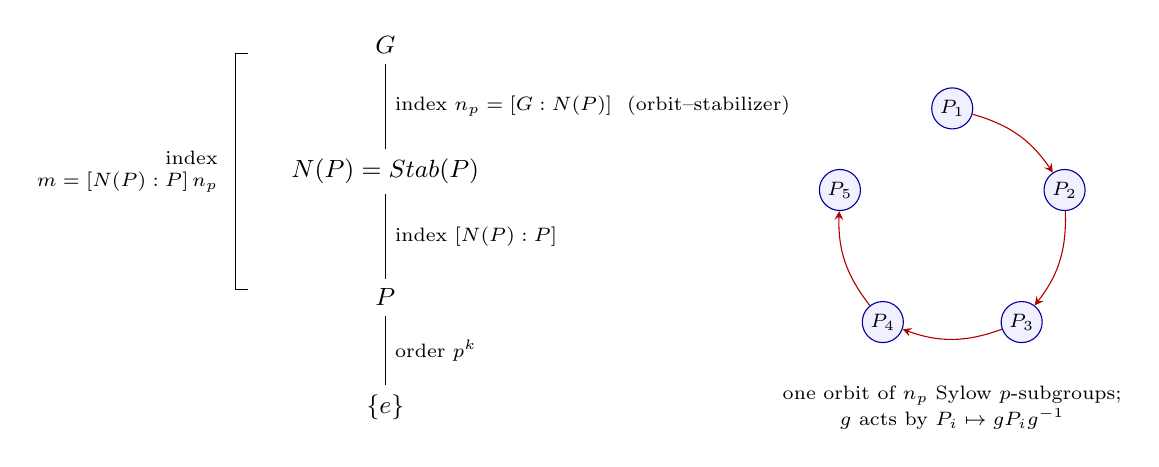
\begin{tikzpicture}[>=stealth, font=\small]
    \node (G) at (0,3.2) {$G$};
    \node (N) at (0,1.6) {$N(P) = \operatorname{Stab}(P)$};
    \node (P) at (0,0) {$P$};
    \node (e) at (0,-1.4) {$\{e\}$};
    \draw (G) -- node[right, font=\scriptsize] {index $n_p = [G : N(P)]$ \ (orbit--stabilizer)} (N);
    \draw (N) -- node[right, font=\scriptsize] {index $[N(P) : P]$} (P);
    \draw (P) -- node[right, font=\scriptsize] {order $p^k$} (e);
    \draw (-1.75,3.1) -- (-1.9,3.1) -- node[left=3pt, font=\scriptsize, align=right] {index\\ $m = [N(P):P]\, n_p$} (-1.9,0.1) -- (-1.75,0.1);
    \begin{scope}[xshift=7.2cm, yshift=0.9cm]
        \foreach \a/\l in {90/P_1, 18/P_2, -54/P_3, -126/P_4, 162/P_5} {
            \node[circle, draw=blue!60!black, fill=blue!6, inner sep=1.5pt, font=\scriptsize] (\l) at (\a:1.5) {$\l$};
        }
        \draw[->, red!70!black, bend left=20] (P_1) to (P_2);
        \draw[->, red!70!black, bend left=20] (P_2) to (P_3);
        \draw[->, red!70!black, bend left=20] (P_3) to (P_4);
        \draw[->, red!70!black, bend left=20] (P_4) to (P_5);
        \node[font=\scriptsize, align=center] at (0,-2.3) {one orbit of $n_p$ Sylow $p$-subgroups;\\ $g$ acts by $P_i \mapsto gP_ig^{-1}$};
    \end{scope}
\end{tikzpicture}
